\documentclass[12pt,a4paper]{article}
\usepackage[utf8]{inputenc}
\usepackage[spanish]{babel}
\usepackage{amsmath}
\usepackage{amsfonts}
\usepackage{amssymb}
\usepackage{graphicx}
\usepackage{kpfonts}
\usepackage[left=2cm,right=2cm,top=2cm,bottom=2cm]{geometry}
\title{EV 2-1 Diseño del puente H\\

\includegraphics [scale=1]{imagenes/UPZMG.png} 
\author{Giovanni Daniel Ruiz Tinoco\\
Alan Antonio Muñoz Juarez\\
\small Sistemas electrónicos de interfaz\\
  \small Universidad Politécnica de la zona metropolitana de Guadalajara\\
  \small 4-B \\
  \small Ing. Mecatrónica\\
\centering
}
}
\begin{document}
\maketitle
\newpage
\begin{center}
\section {MARCO TEÓRICO}
\end{center}
\subsection{¿Qué es un puente H?}
El puente H  es un circuito electrónico que permite a un motor eléctrico DC girar en ambos sentidos, avanzar y retrocerder.

Los puentes H ya vienen hechos en algunos circuitos integrados, pero también se pueden construir a partir de componentes eléctricos y/o electronicos.

Un puente H se construye con 4 interruptores (mécanicos o mediante transistores). Cuando los interruptores S1 y S4 están cerrados ( S2 y S3 abiertos ) se aplica una tensión haciendo girar el motor en un sentido. Abriendo los interruptores S1 y S4 ( cerrando S2 y S3 ), el voltaje se invierte, permitiendo el giro en sentido inverso del motor.
\begin{center}
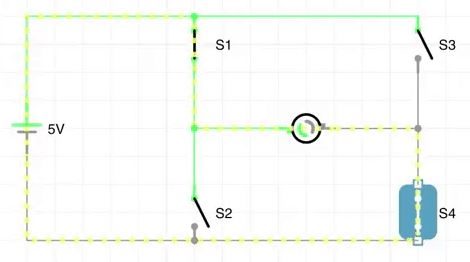
\includegraphics[scale=1]{imagenes/gg.jpg}  
\end{center}
\begin{flushleft}
Un puente H no solo se usa para invertir el giro de un motor, también se puede usar para frenarlo de manera brusca, al hacer un corto entre los bornes del motor, o incluso puede usarse para permitir que el motor frene bajo su propia inercia, cuando desconectamos el motor de la fuente que lo alimenta.\linebreak

básicamente se puede hacer esto tomando en cuenta la siguiente tabla.\linebreak
\begin{center}
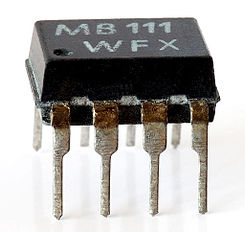
\includegraphics[scale=0.5]{imagenes/opto.JPG}
\end{center}
\end{flushleft}
\newpage
\subsection{Jfet}
\begin{flushleft}
El principio de utilizar un campo eléctrico para controlar el flujo de corriente se introdujo con el desarrollo del transistor BJT , por otro lado, los transistores de Efecto de Campo o Field Effect Transistors (FETs) es un dispositivo controlado por voltaje, estos son artefactos unipolares, o sea que en el proceso de conducción utilizan electrones o huecos y no ambos como los BJT.\linebreak
\begin{center}
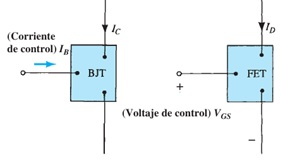
\includegraphics[scale=1.0]{imagenes/jfet.JPG}\linebreak
\end{center}
El FET consiste de un semiconductor dopado (canal) con dos terminales en los extremos llamados Source y Drain. La corriente en el canal (entre Drain y Source) es controlada por el voltaje en un tercer terminal llamado Gate.
Los FETs se dividen en tres categorías principales:  el transistor de efecto de campo de unión (JFET), el transistor de efecto de campo semiconductor de óxido metálico (MOSFET), y el transistor de efecto de campo semiconductor metálico (MESFET). La categoría MOSFET se divide aún más en tipos de empobrecimiento y enriquecimiento. \linebreak
\begin{center}
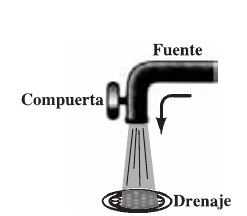
\includegraphics[scale=1.0]{imagenes/jfet1.JPG}\linebreak
\end{center}
El transistor MOSFET ha llegado a ser uno de los dispositivos más importantes utilizados en el diseño y construcción de circuitos integrados para computadoras digitales. Sin embargo, por ser un elemento discreto confinado en un contenedor acopado, requiere un manejo cuidadoso. El MESFET es un desarrollo más reciente y aprovecha al máximo la ventaja de las características de alta velocidad del GAs como material semiconductor base. Aun cuando en la actualidad es la opción más cara, el tema del costo a menudo es superado por la necesidad de mayores velocidades en diseños de radiofrecuencia y de computadoras.\linebreak
Al igual que los BJT, los FETs son interruptores de dos semirectas en el mismo cuadrante y, en consecuencia, con encendido y apagado controlados, pero se distinguen de éstos porque la corriente de salida está controlada por un voltaje. Las ventajas de los FETs con respecto a los BJT incluyen menos ruido, mayor estabilidad termal, mayor disipación de potencia y que pueden sostener corrientes muy altas, entre las desvantajas se encuentran una pobre respuesta de frecuencia debido a la alta capacitancia de entrada y a que se dañan fácilmente con la electricidad estática.\linebreak
\begin{center}
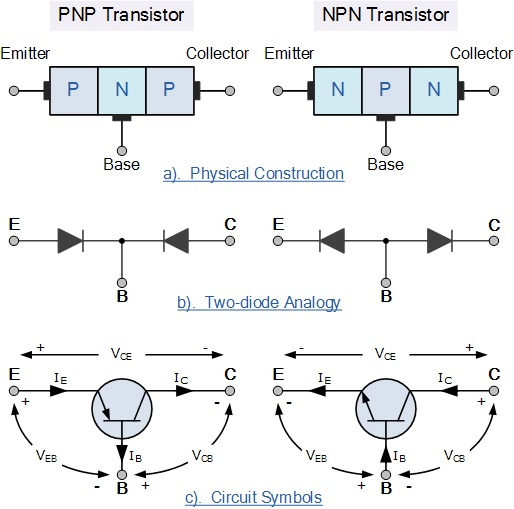
\includegraphics[scale=1.0]{imagenes/jfet0.jpg}\linebreak
\end{center}
\end{flushleft}
\newpage
\begin{flushleft}
\begin{center}
\section{Procedimiento}
\end{center}
\subsection{Materiales}
\end{flushleft}
\begin{flushleft}
1. Computadora\linebreak
2. Fuente de voltaje\linebreak
3. Mosfet IF640/840\linebreak
4. Arduino\linebreak
5. Circuito simulador de PLC controlado por arduino\linebreak
6. Motor DC\linebreak
\linebreak
Realice la simulación y el circuito del siguiente esquema:\\
\end{flushleft}
\begin{center}
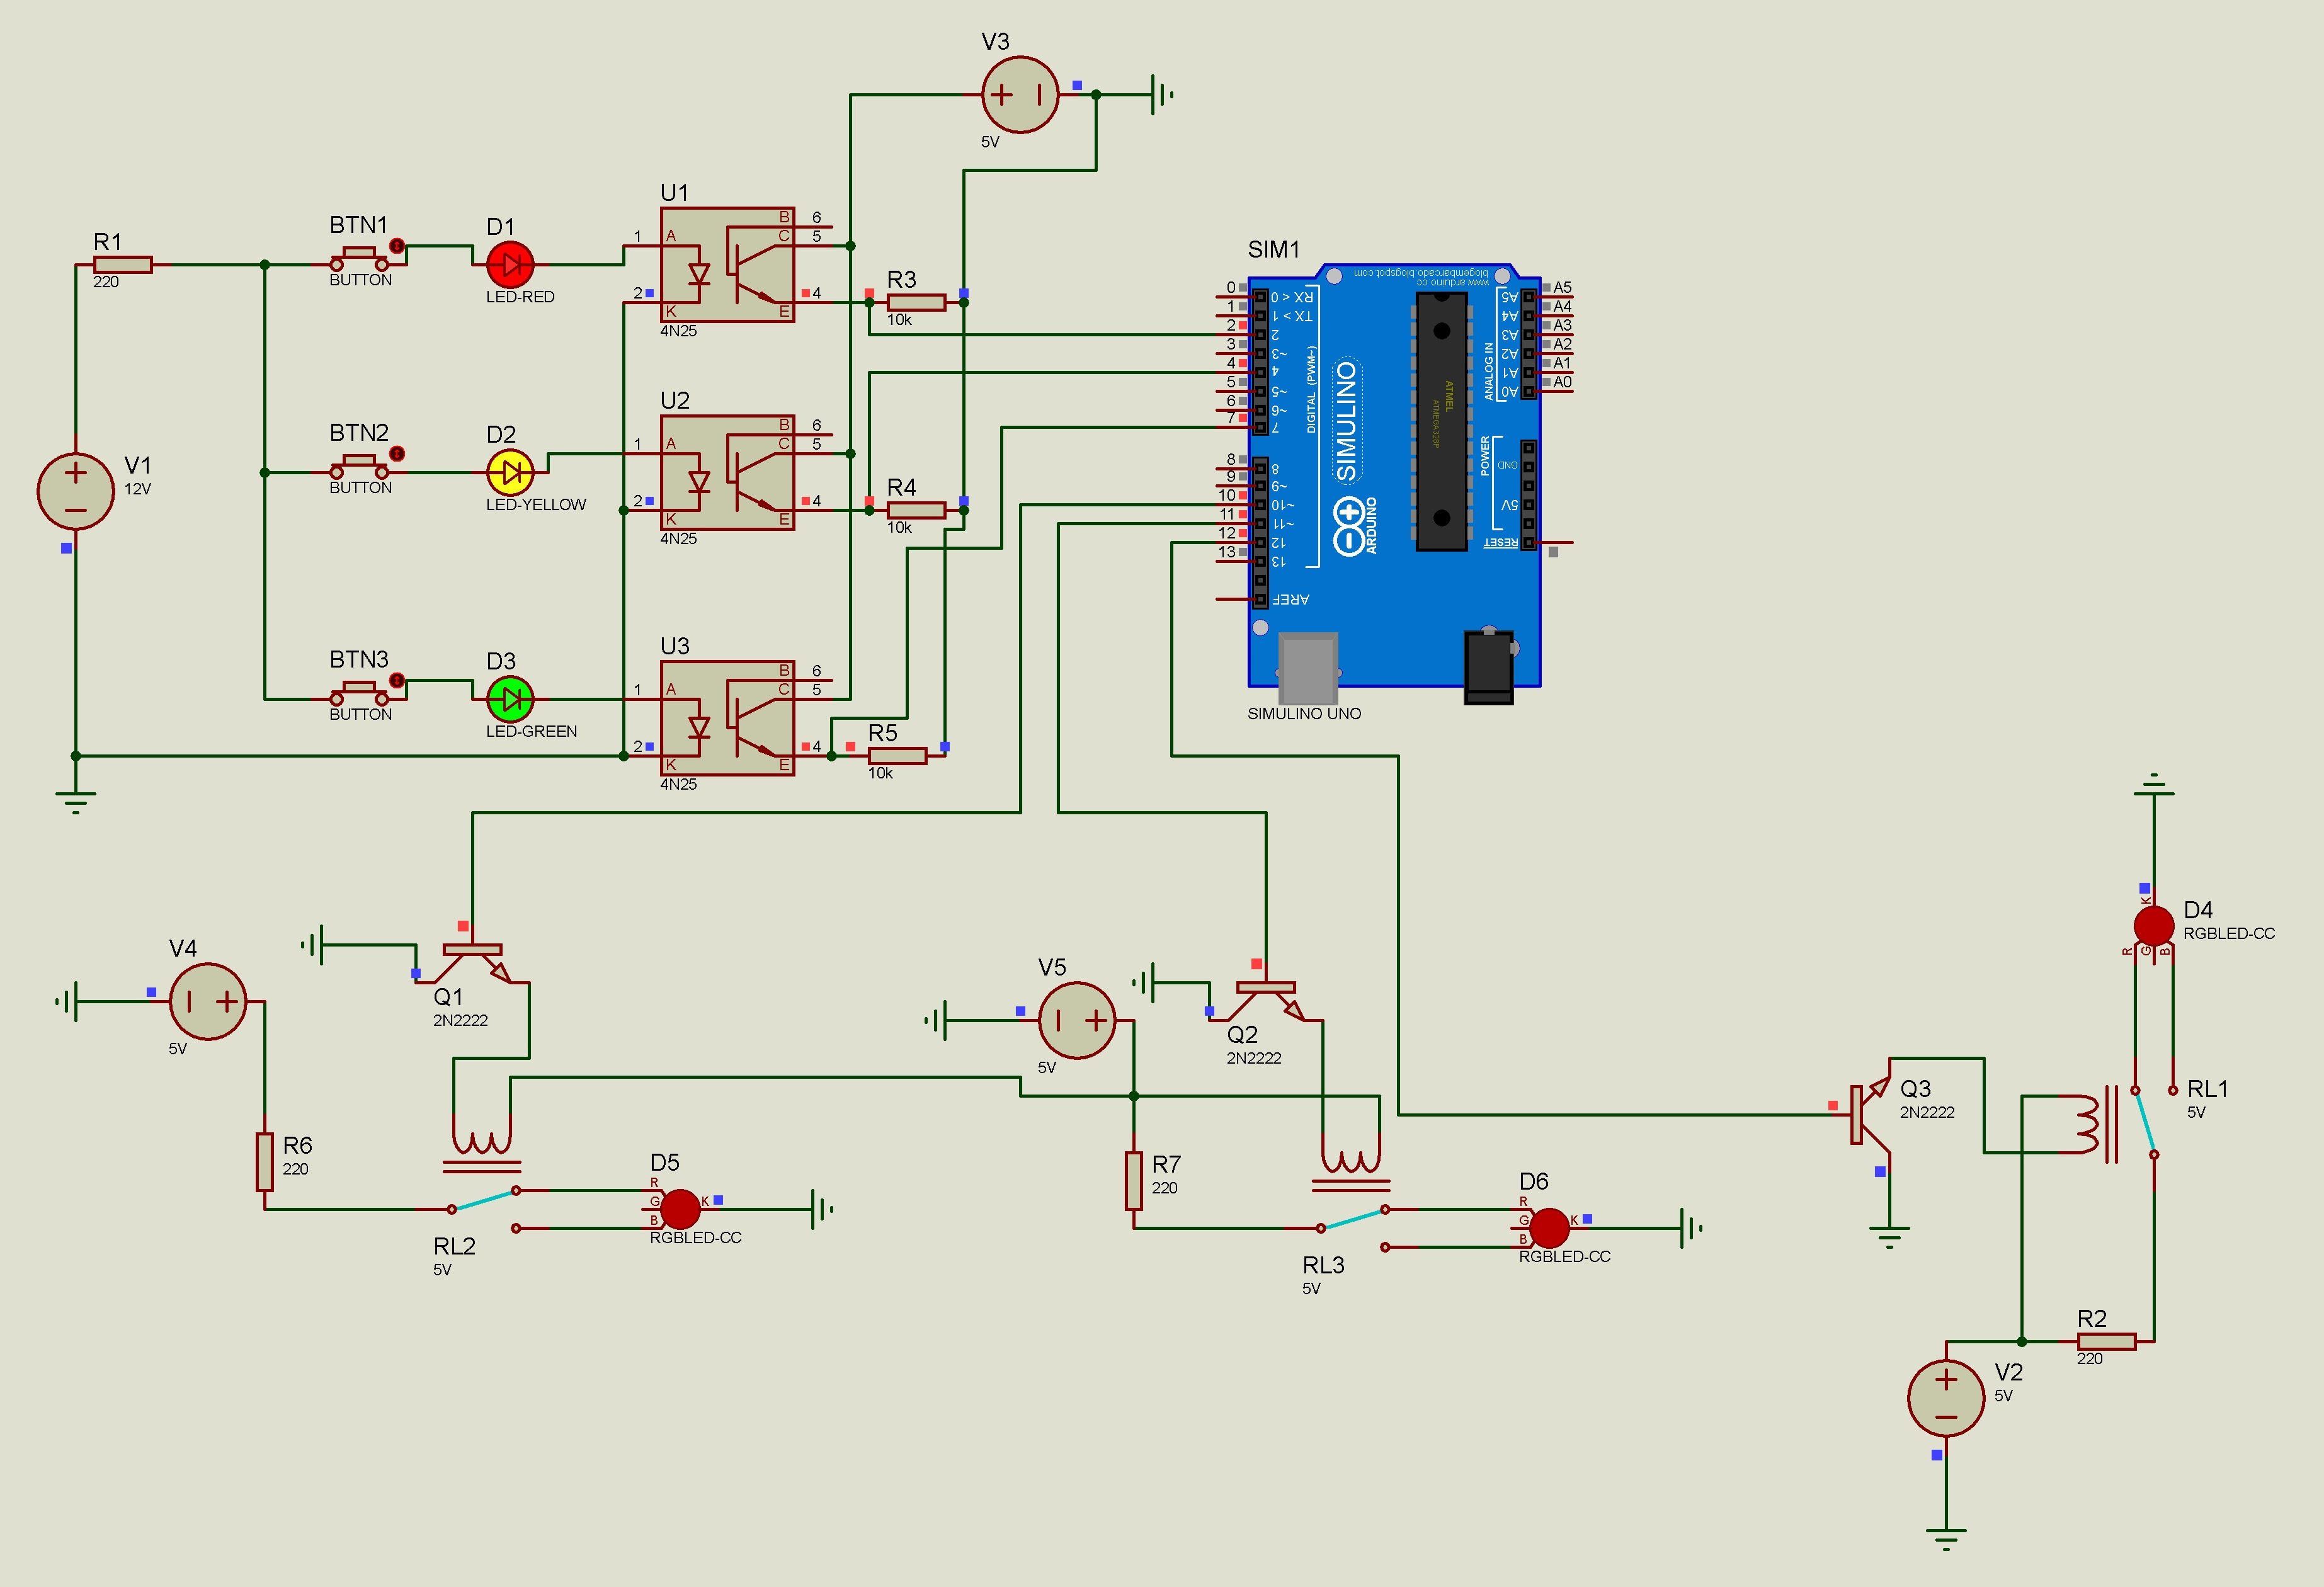
\includegraphics[scale=0.22]{imagenes/simu0.JPG}\linebreak
\end{center}
\newpage
\begin{flushleft}
\subsection{Desarrollo de la práctica}
Primero armaremos el puente H basandonos en el circuito a continuación:\linebreak
\begin{center}
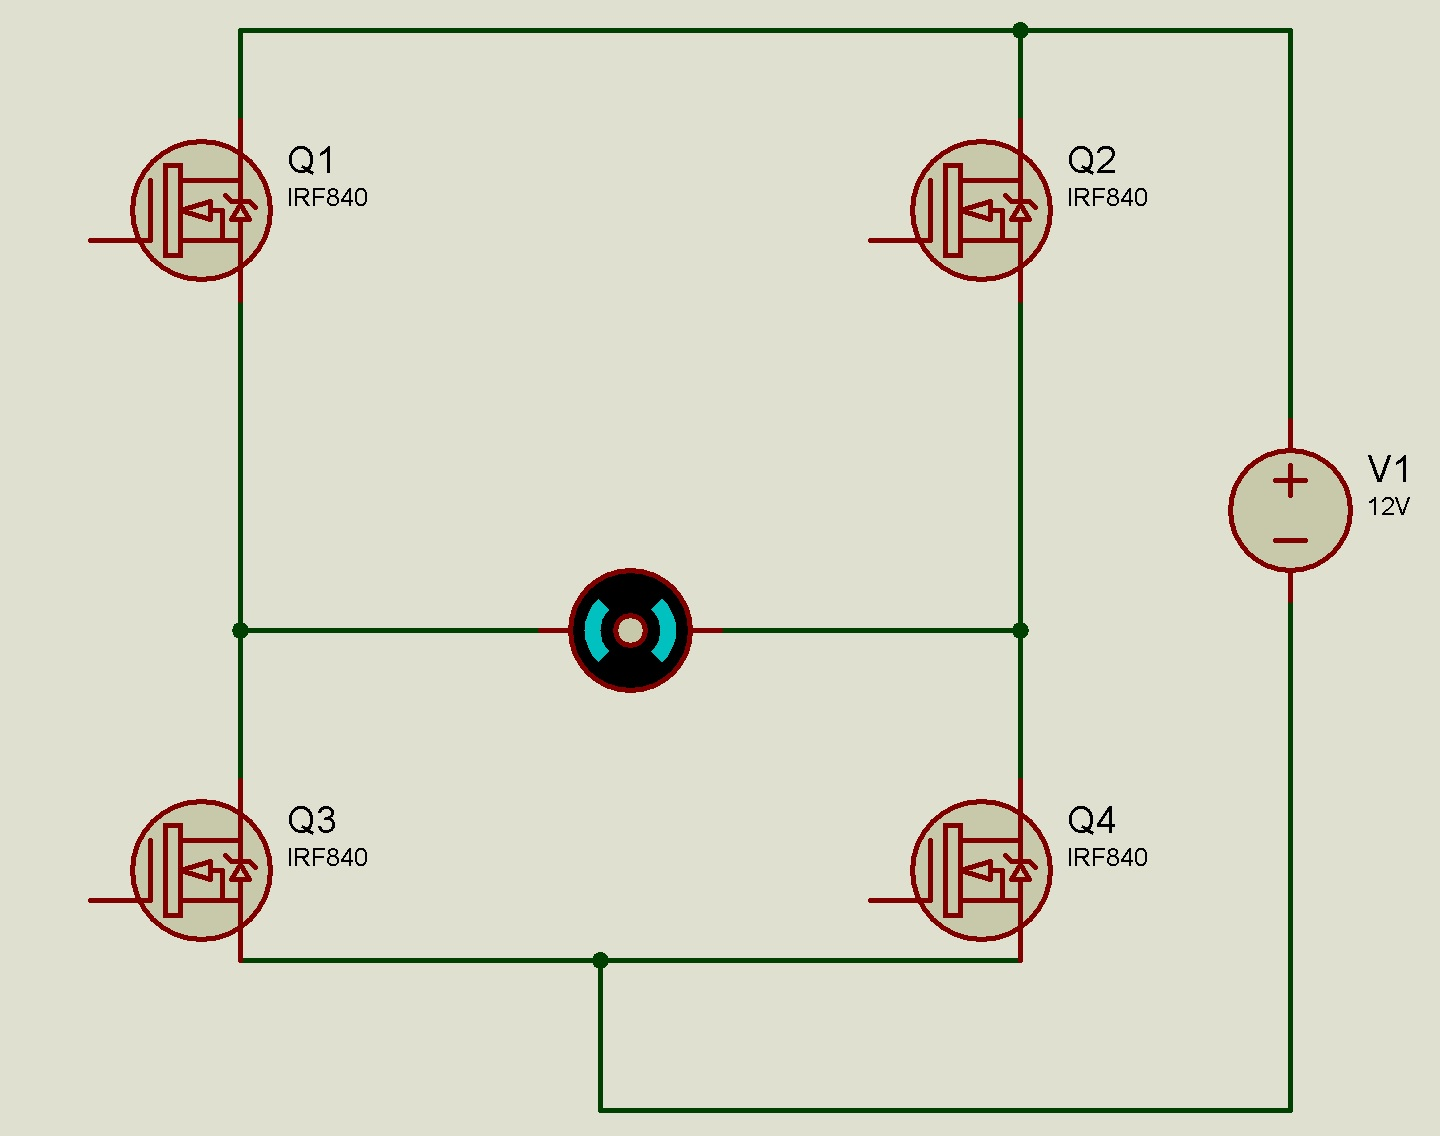
\includegraphics[scale=0.22]{imagenes/simu1.JPG}\linebreak
\end{center}
El resultado final debe ser similar al de la siguiente imagen:\linebreak
\begin{center}
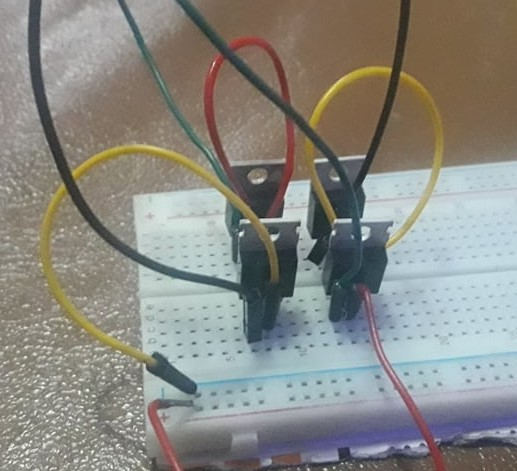
\includegraphics[scale=1]{imagenes/fefe2.JPG}\linebreak
\end{center}
\newpage
Ahora vamos a conectar el puente H con el circuito que hemos trabajado en practicas anteriores este tiene la función de simular un PLC, lo que haremos sera conectar los intercalados para que así el motor pueda girar en ambas direcciones por que al activarse la polaridad de la alimentación motor se va a invertir.\linebreak
\linebreak
Para realizar la conexion nos basaremos en el circuito que ya habíamos armado:\linebreak
\begin{center}
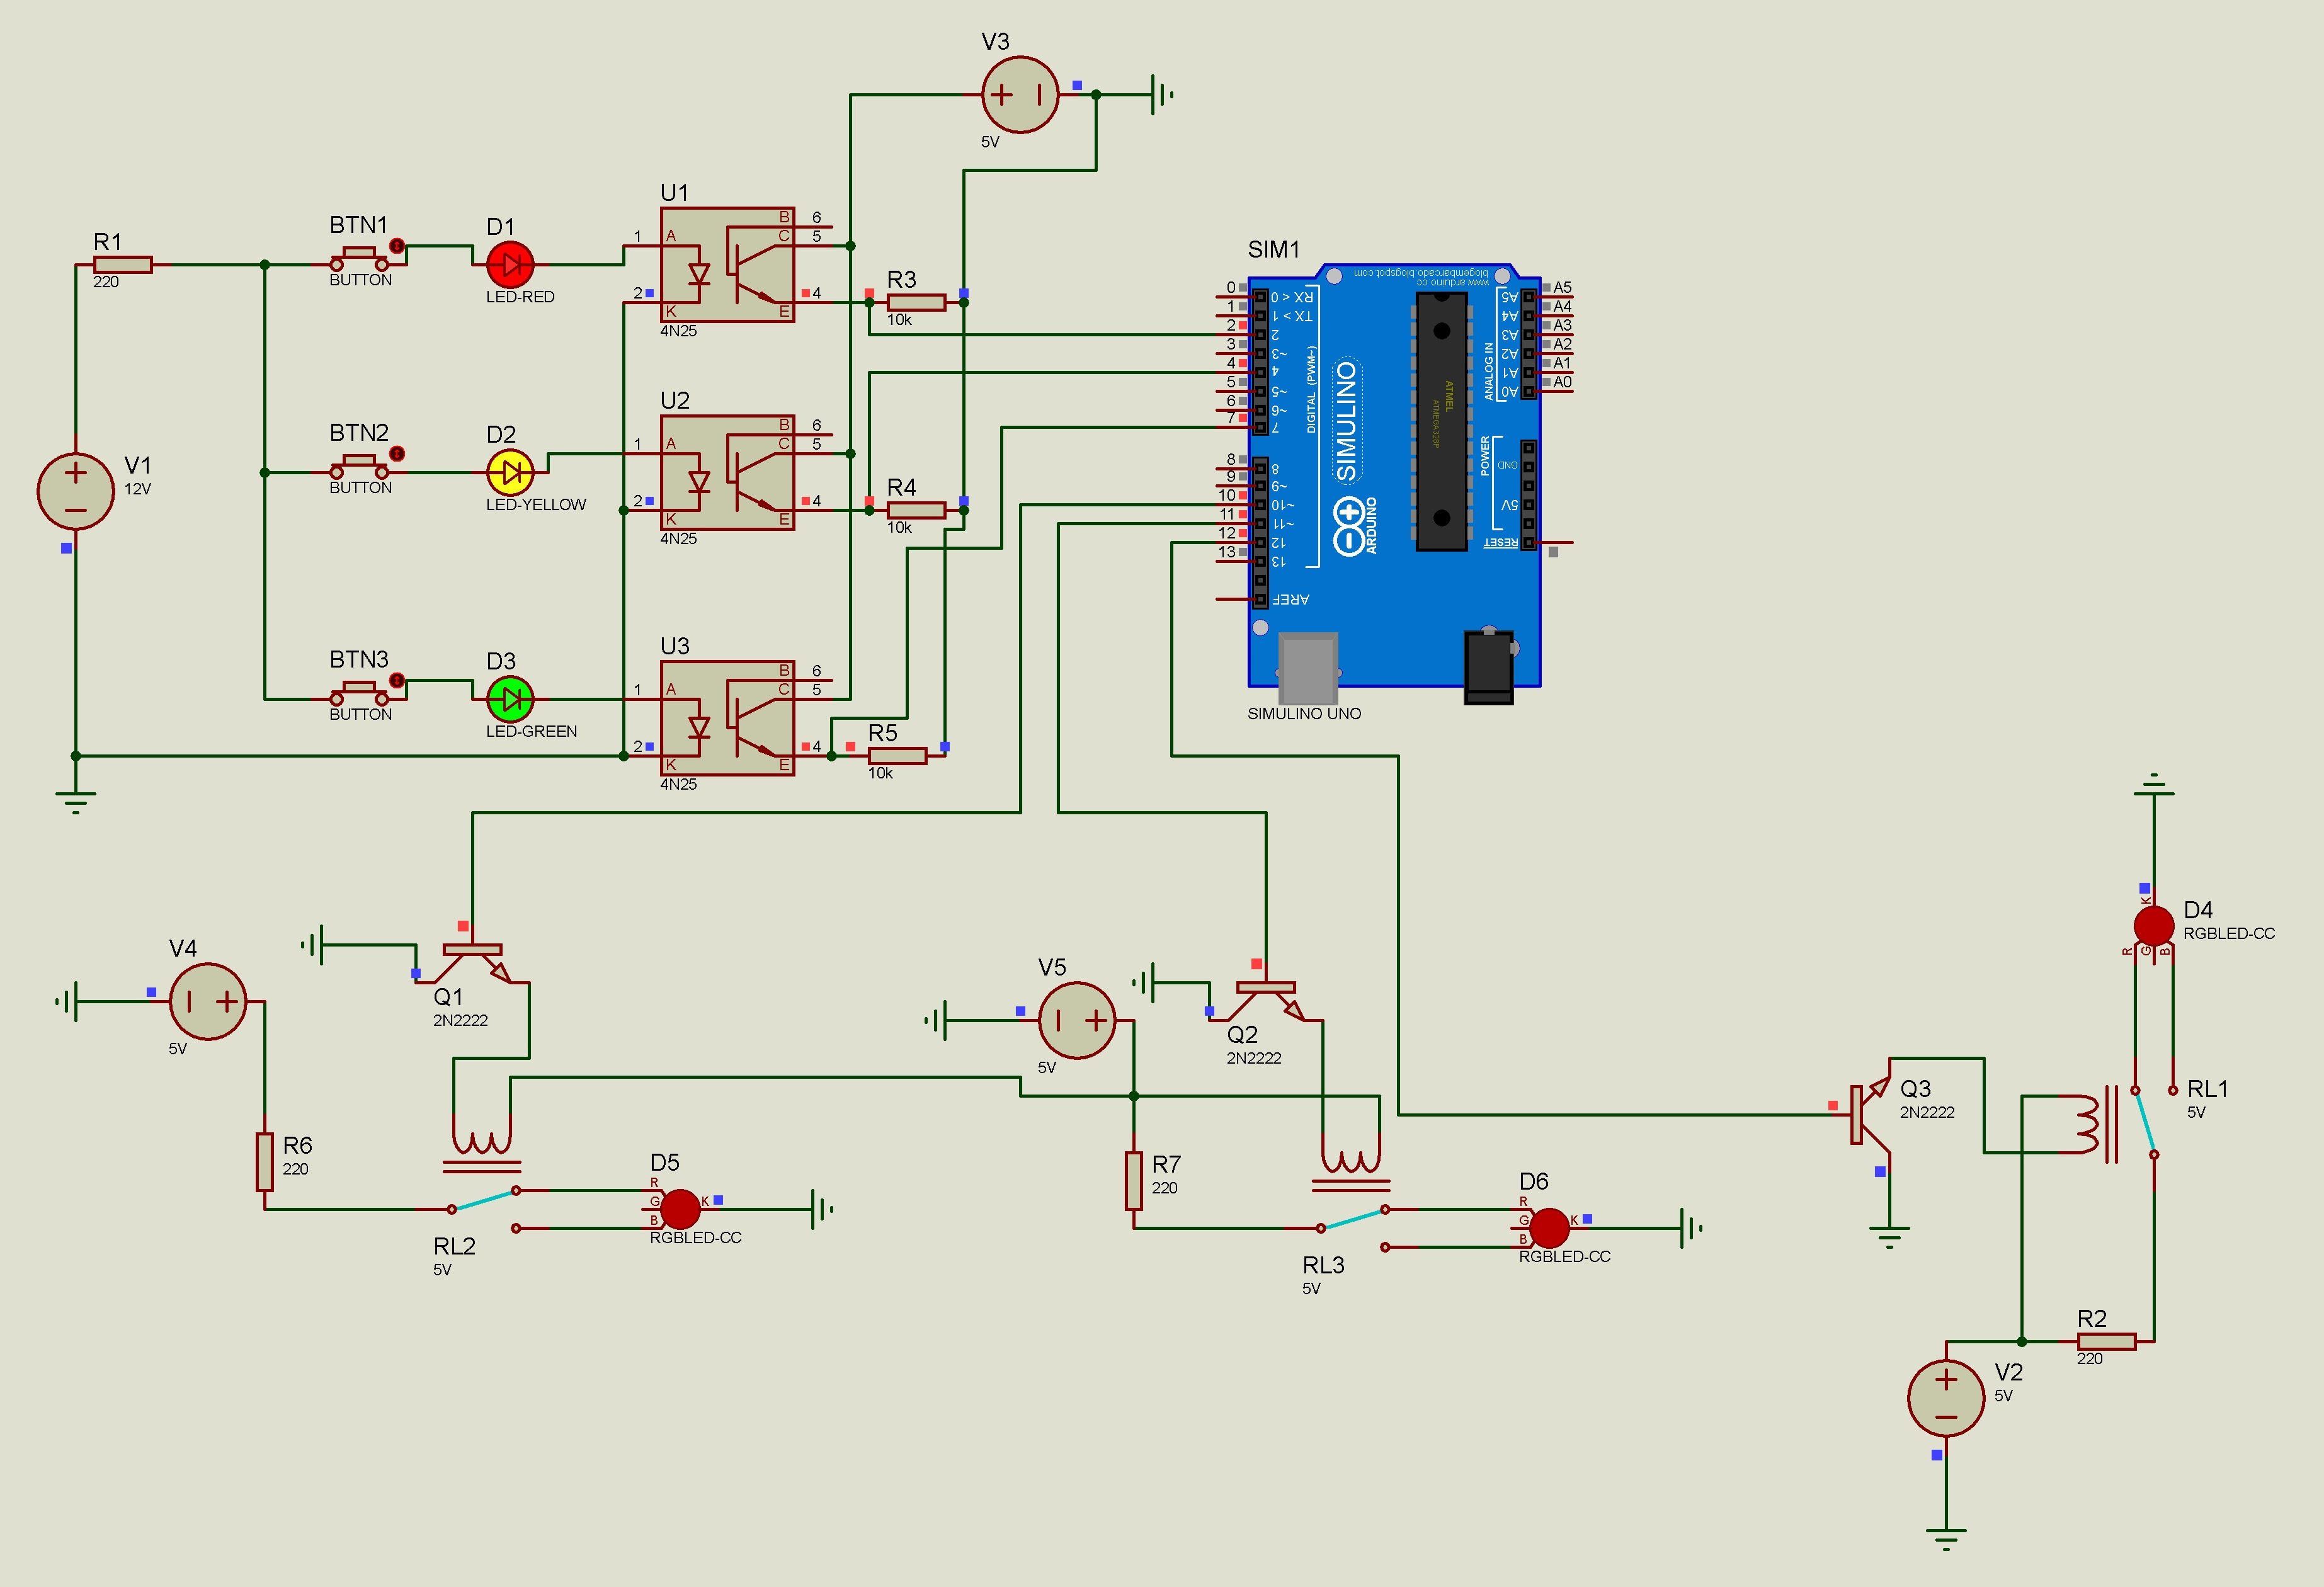
\includegraphics[scale=0.2]{imagenes/simu0.JPG}\linebreak
\end{center}
Finalmente el circuito debe quedar de la siguiente manera ya armado y realizando la función antes descrita:\linebreak

\begin{center}
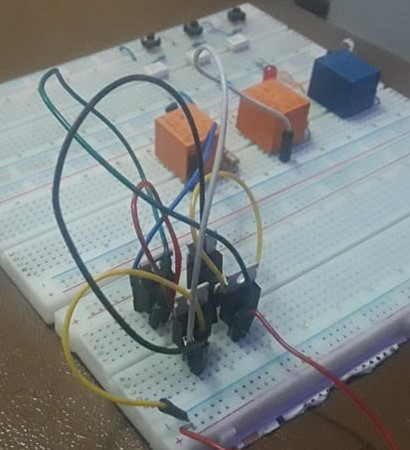
\includegraphics[scale=0.7]{imagenes/fefe0.JPG}\linebreak
\end{center}
\end{flushleft}
\newpage
\begin{flushleft}
\section{Producto final}
Ya con el circuito armado solo debemos presionar un boton u otro para hacer que el motor gire en una u otra dirección controlado por el puente H.\linebreak

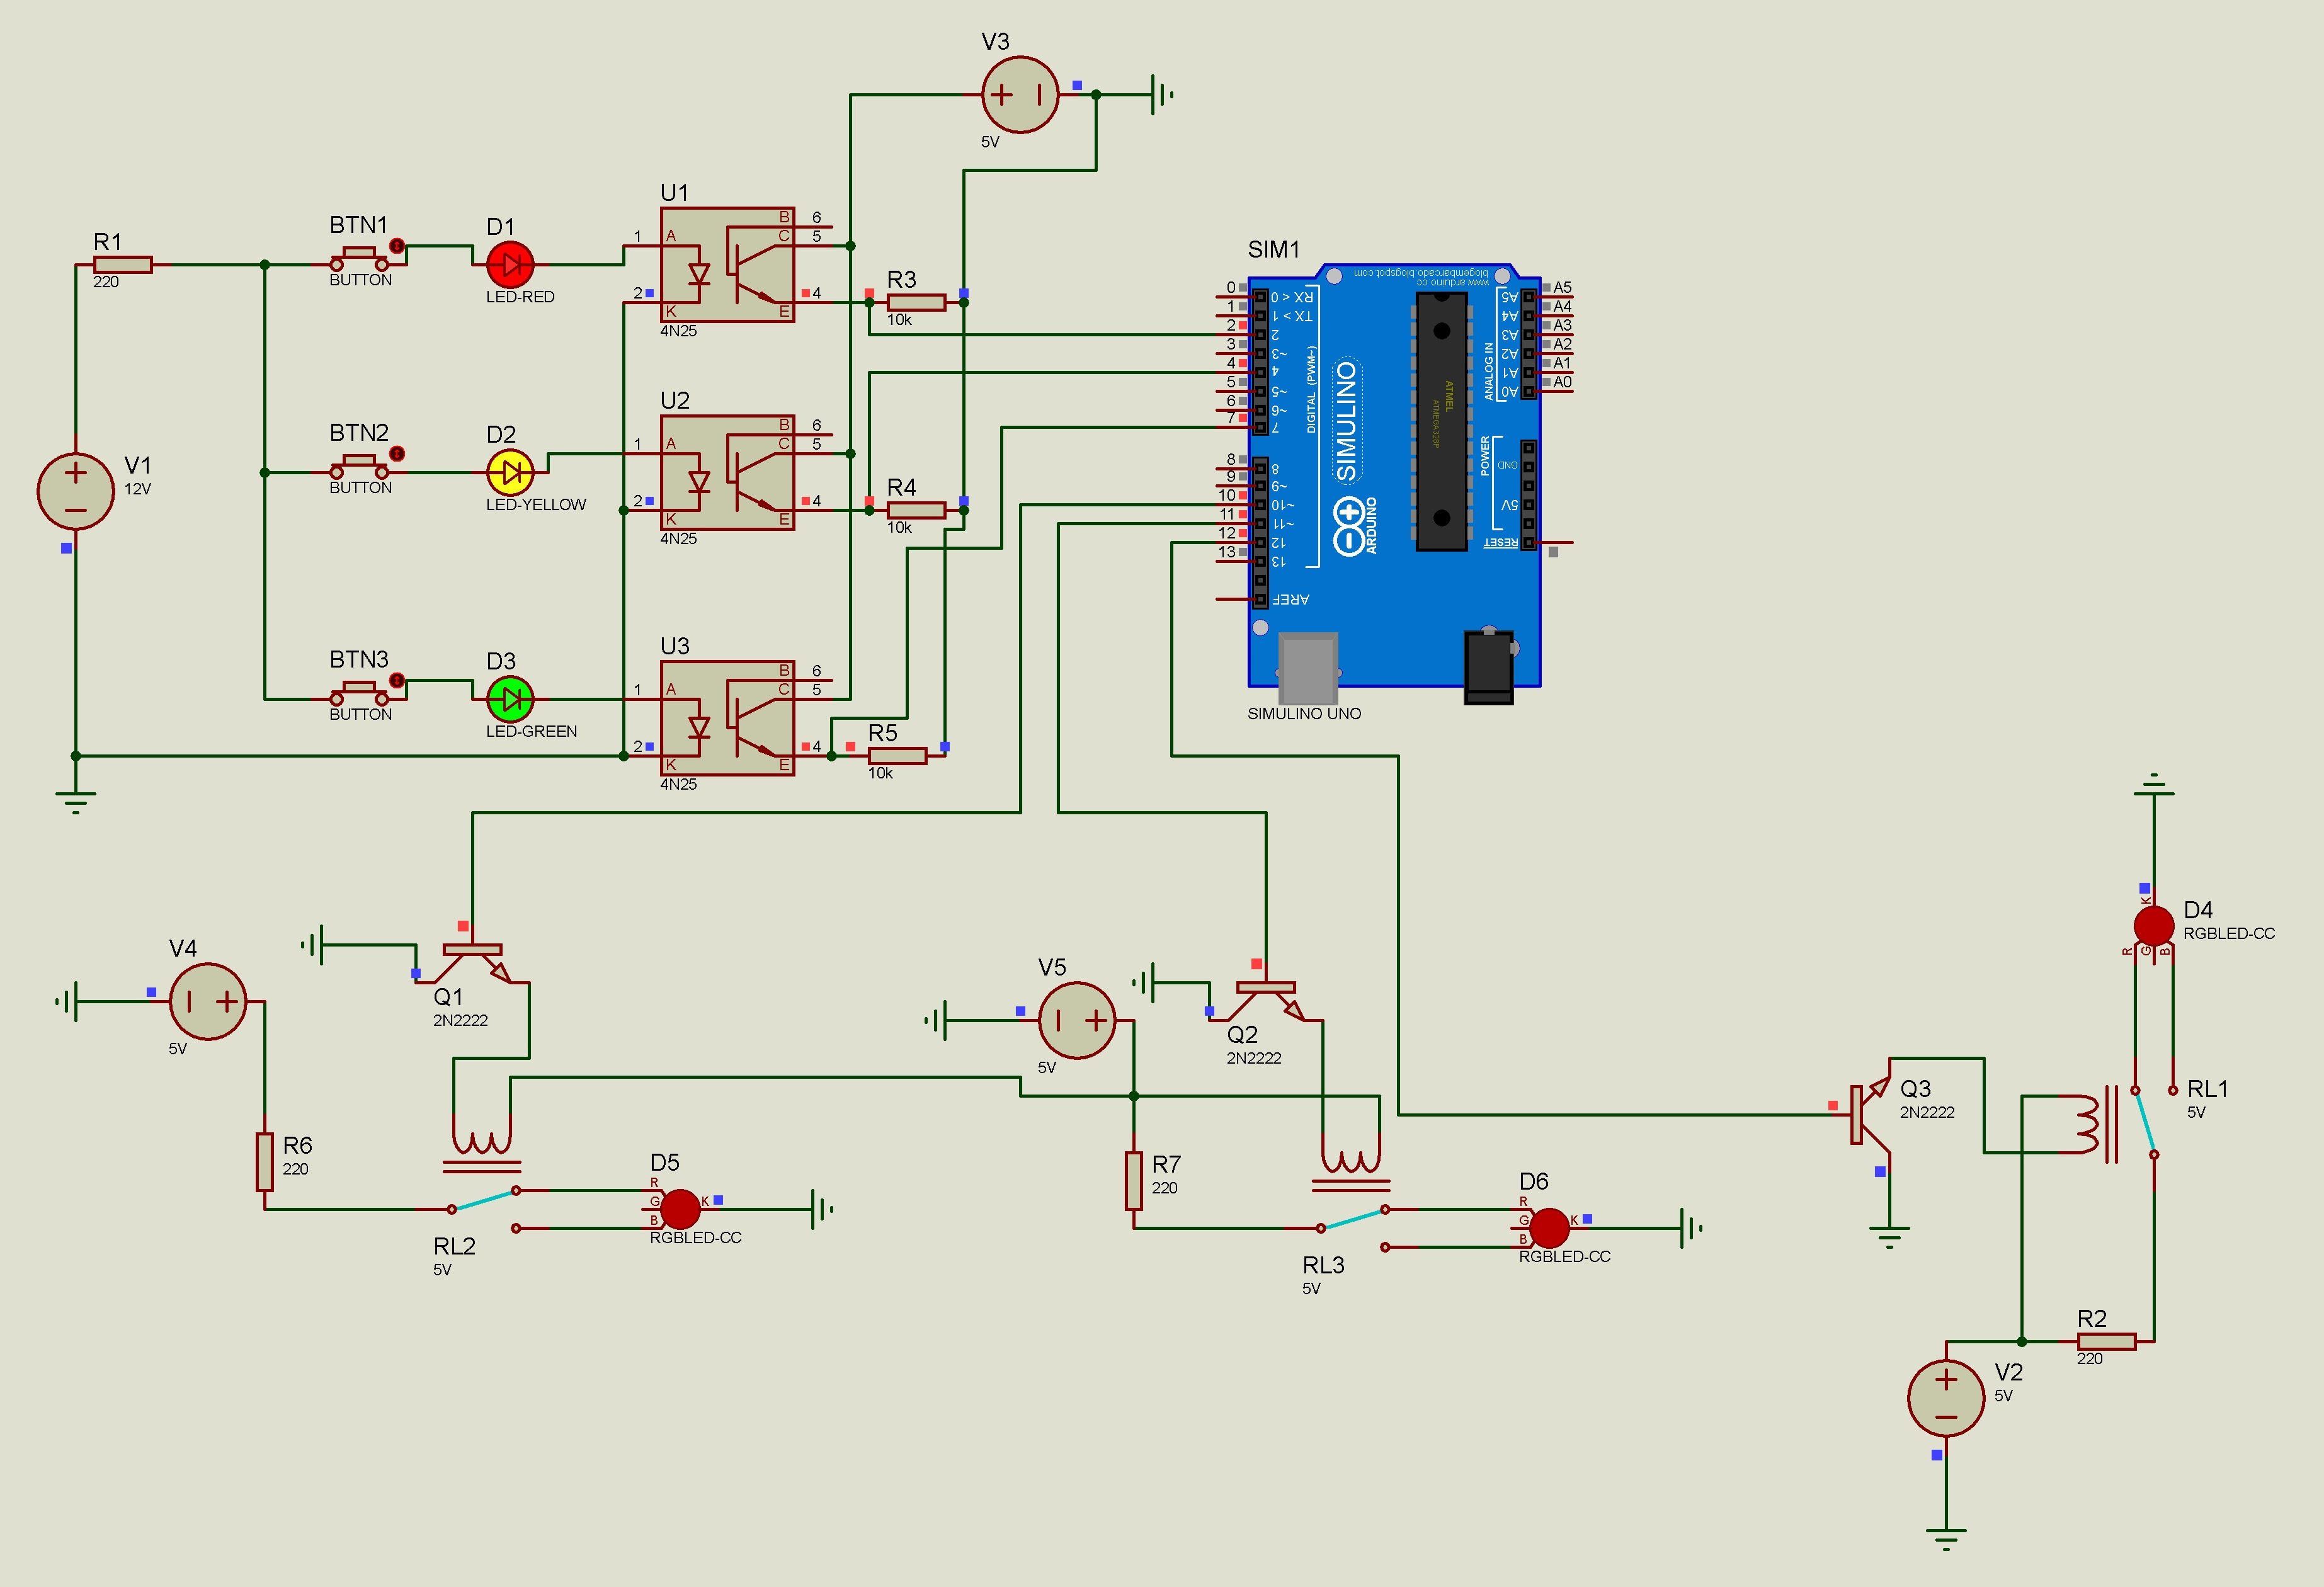
\includegraphics[scale=0.2]{imagenes/simu0.JPG}\linebreak

\section{Conclusión}
Los mosfets hace la función de un interruptor en el circuito permitiendo la polarizacion en ambos sentidos,estos componentes son de gran importancia en la industria ya que ellos puede manejar corrientes bastante grandes son usados mucho para la  de partes que necesitan  de amperaje para funcionar por ello son de gran importancia en nuestra carrera que esta enfocada a la automatización de sistemas.

\section{Bibliográfia}
INVENTABLE.(2017).Cómo funciona un puente para motores de corriente continua. 16/10/19, de inventable Sitio web: https://www.inventable.eu/2017/05/26/funciona-puente-motores-corriente-continua\linebreak

Frank Mecafenix . (2017). ¿Qué es un puente H?. 16/10/19, de Ingeniería Mecafenix Sitio web: https://www.ingmecafenix.com/electronica/puente-h-control-motores/\linebreak

Antony García. (2016). ¿Qué es y cómo se utiliza un MOSFET?. 16/10/19, de Panahitex Sitio web: http://panamahitek.com/que-es-y-como-funciona-un-mosfet/\linebreak

\end{flushleft}

\end{document}
\section{se}